\section{Présentation du projet}

\subsection{Screenshot}
{
\logo{}
\begin{frame}
\frametitle{Présentation du projet}
\begin{center}
    \begin{figure}[h!]
        \vspace*{-1.5em}
        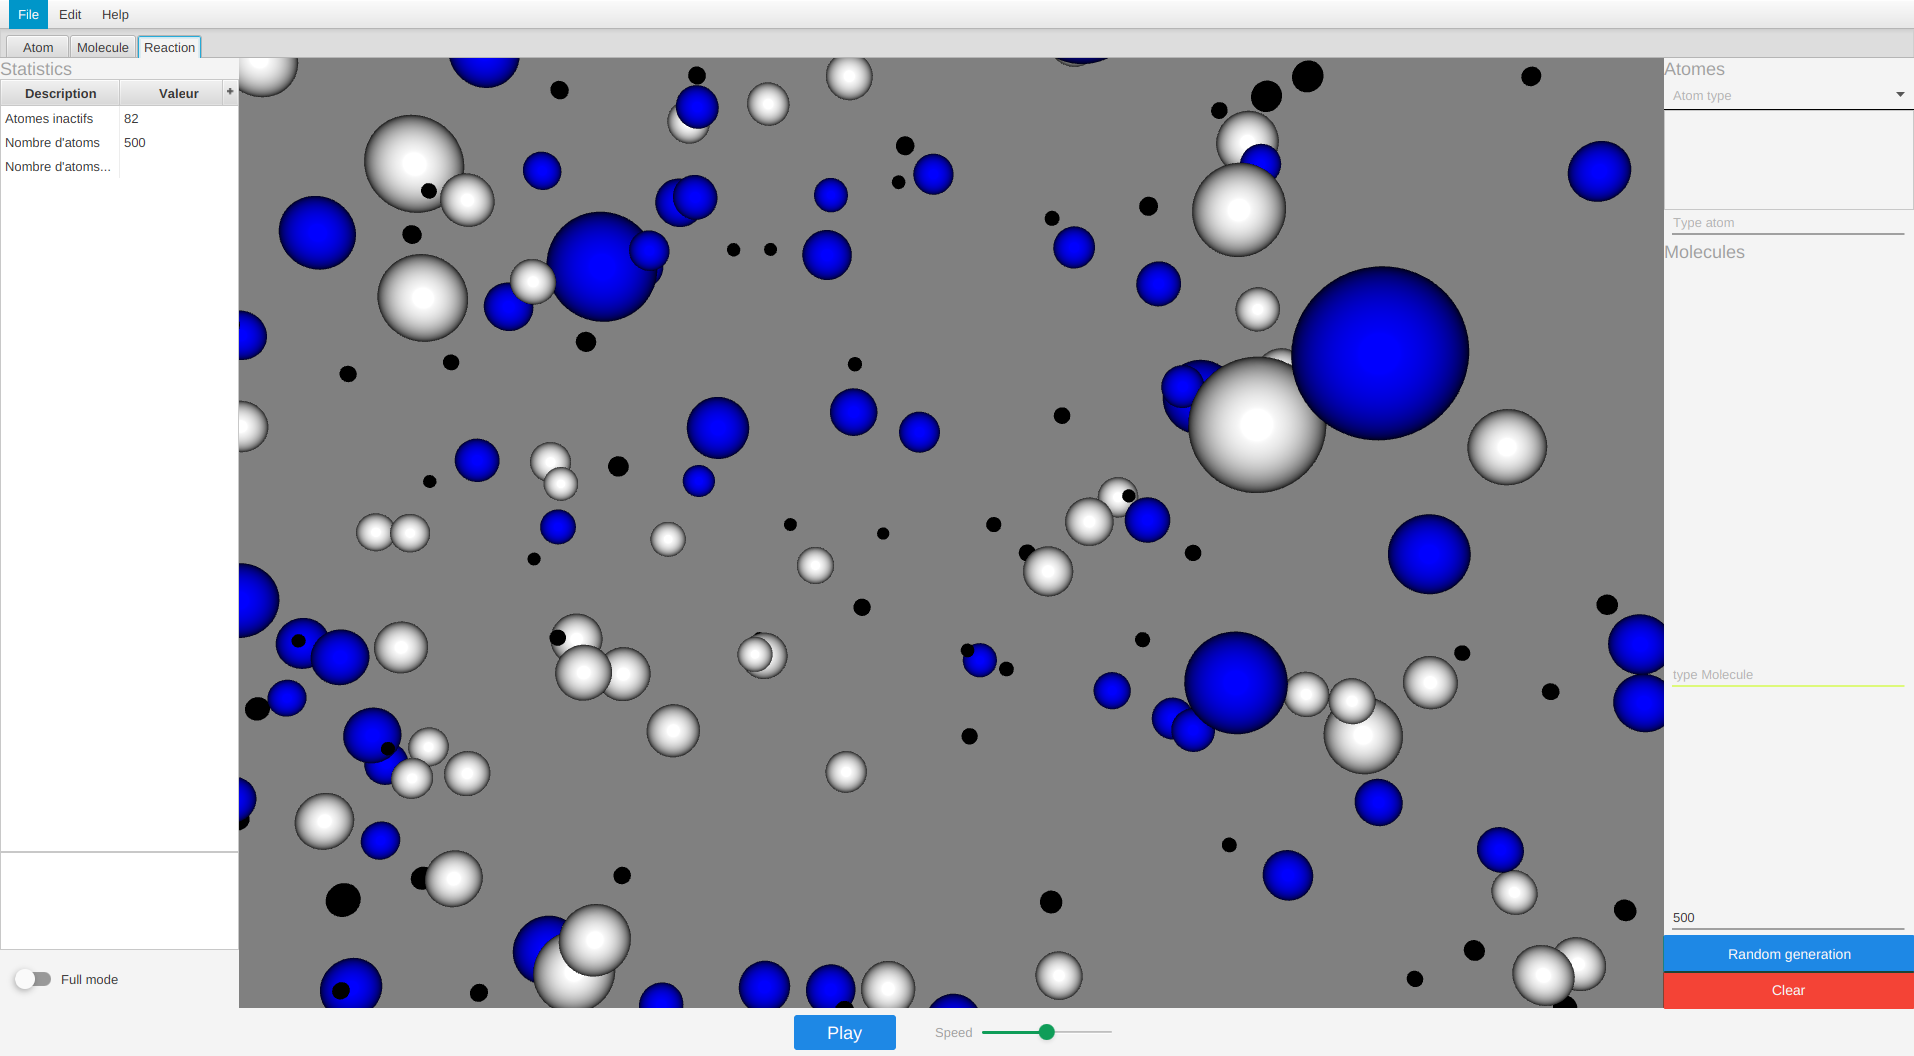
\includegraphics[width=115mm]{screenshot_app}
    \end{figure}
\end{center}
\end{frame}
}

\subsection{Modules de l'application}

\begin{frame}
\frametitle{Les modules de l'application}
\begin{center}
\definecolor{mygray}{RGB}{208,208,208}
\definecolor{mymagenta}{RGB}{226,0,116}
\newcommand*{\mytextstyle}{\sffamily\Large\bfseries\color{black!85}}
\newcommand{\arcarrow}[3]{%
   % inner radius, middle radius, outer radius, start angle,
   % end angle, tip protusion angle, options, text
   \pgfmathsetmacro{\rin}{1.7}
   \pgfmathsetmacro{\rmid}{2.2}
   \pgfmathsetmacro{\rout}{2.7}
   \pgfmathsetmacro{\astart}{#1}
   \pgfmathsetmacro{\aend}{#2}
   \pgfmathsetmacro{\atip}{5}
   \fill[mygray, very thick] (\astart+\atip:\rin)
                         arc (\astart+\atip:\aend:\rin)
      -- (\aend-\atip:\rmid)
      -- (\aend:\rout)   arc (\aend:\astart+\atip:\rout)
      -- (\astart:\rmid) -- cycle;
   \path[
      decoration = {
         text along path,
         text = {|\mytextstyle|#3},
         text align = {align = center},
         raise = -1.0ex
      },
      decorate
   ](\astart+\atip:\rmid) arc (\astart+\atip:\aend+\atip:\rmid);
}
\begin{tikzpicture}
   \fill[even odd rule,mymagenta] circle (1.5);

   \node at (0,0) [
      font  = \mytextstyle,
      color = white,
      align = center
   ]{
      Atom\\
      Simulator
   };
   \arcarrow{ 85}{3}{ Atomic  }
   \arcarrow{270}{357}{ Molecular }
   \arcarrow{90}{269}{ Reaction }
\end{tikzpicture}
\end{center}
\end{frame}
